\section{Interazioni di corrente neutra}
Ricaviamo adesso le formule per le sezioni d'urto di neutrini (e antineutrini) in processi di corrente neutra su nucleone
$$
\nu_\mu N \rightarrow \nu_\mu X \qquad \bar{\nu}_\mu N \rightarrow \bar{\nu}_\mu X
$$
Vogliamo sviluppare le formule nell'ambito del modello a partoni e ci servono le sezioni d'urto per interazioni di neutrini su quark. Una formulazione analoga a quella delle correnti cariche ci porta ad ipotizzare un'ampiezza di scattering proporzionale al prodotto di due correnti
$$\mathfrak{M} = \frac{G}{\sqrt{2}}2\rho J_\mu^{NC}(\nu)J_{NC}^\mu(q)$$
\begin{figure}[h!]
	\centering
	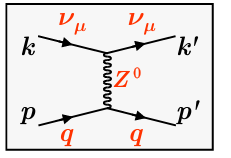
\includegraphics[width=0.3\textwidth]{Lezioni/Lezione 20/salaa1.png}
	\label{fig:salaa1}
\end{figure}
Il parametro $\rho$ tiene conto di un'eventuale differenza di intensità fra la corrente carica (G) e la corrente neutra ($\rho G$). Le correnti cariche hanno mostrato che il neutrino è sempre left-handed: assumiamo che la corrente neutra abbia la stessa forma chirale
$$J_\mu^{NC}(\nu) = \frac{1}{2}\bar{u}_\nu\gamma_\mu(1 - \gamma^5)u_\nu$$
Per la corrente dei quark si assumono sempre gli accoppiamenti vettoriali ($V,A$) ma con coefficienti $c_v$ e $c_a$ arbitrari da determinare
$$J_\mu^{NC}(q) = \frac{1}{2}\bar{u}_q\gamma_\mu(c_v - c_a\gamma^5)u_q$$
L'arbitrarietà di $c_v$ e $c_a$ (che devono essere determinati dall'esperimento) significa che la corrente neutra può contenere una componente $L$ e una $R$. Infatti troviamo $g_R$ e $g_L$ tali che
$$c_v - c_a\gamma^5 = g_R(1 + \gamma^5) + g_L(1 - \gamma^5)$$
Sviluppando
$$\left\{\begin{aligned} g_R + g_L &= c_v \\ g_R - g_L &= -c_a \end{aligned}\right. \qquad $$
$$\left\{\begin{aligned} g_R &= \frac{c_v - c_a}{2} \\ g_L &= \frac{c_v + c_a}{2} \end{aligned}\right.$$
Infine
$$J_\mu^{NC}(q) = \frac{1}{2}g_R\bar{u}_q\gamma_\mu(1 + \gamma^5)u_q + \frac{1}{2}g_L\bar{u}_q\gamma_\mu(1 - \gamma^5)u_q$$
Pertanto l'elemento di matrice diventa
$$\mathfrak{M} = \frac{4G}{\sqrt{2}}2\rho J_\mu^{NC}(\nu)J_{NC}^\mu(q) = \frac{4G}{\sqrt{2}}2\rho\left[g_L J_\mu^{NC}(\nu)J_{NC}^\mu(q_L) + g_R J_\mu^{NC}(\nu)J_{NC}^\mu(q_R)\right]$$
La somma dell'ampiezza di scattering di un neutrino:
\begin{itemize}
	\item Su un quark Right Handed $q_R$ con intensità $g_R$
	\item Su un quark Left Handed $q_L$ con intensità $g_L$
\end{itemize}
\section{Interazione neutrino quark (NC)}
La sezione d'urto per l'interazione neutrino-quark tramite corrente neutra possono essere scritte utilizzando i risultati ottenuti per le correnti cariche. Dal momento che la corrente neutra è una sovrapposizione di una corrente $V-A$ e di una corrente $V+A$ per ogni sezione d'urto occorre considerare due contributi. Abbiamo inoltre visto che la dipendenza della sezione d'urto dell'angolo era determinata dalle elicità dei fermioni e dal momento angolare totale. La sezione d'urto è isotropa quando $J_z=0$ nei casi $\nu_\mu q_L$ e $\nu_\mu \bar{q}_R$. La sezione d'urto invece dipende da $(1+\cos(\theta))^2$ per $J_z=\pm1$ nei casi $\nu_\mu q_R$ e $\nu_\mu \bar{q}_L$. Per le interazioni di antineutrini valgono considerazioni analoghe. Infine avevamo utilizzato la relazione
$$
1-y=\frac{1}{2}(1+\cos(\theta))
$$
\begin{figure}[h!]
	\centering
	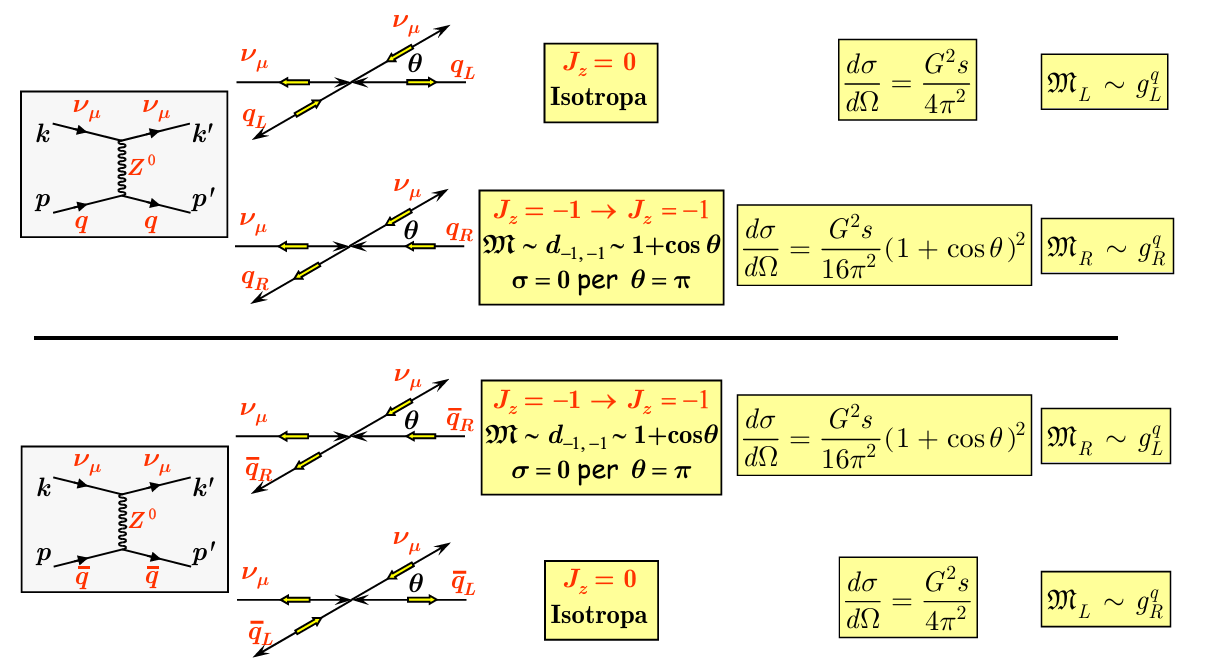
\includegraphics[width=0.9\textwidth]{Lezioni/Lezione 20/salaa2.png}
	\label{fig:salaa2}
\end{figure}
Le sezioni d'urto di anti neutrino sono ragionamenti praticamente opposte
\begin{figure}[h!]
	\centering
	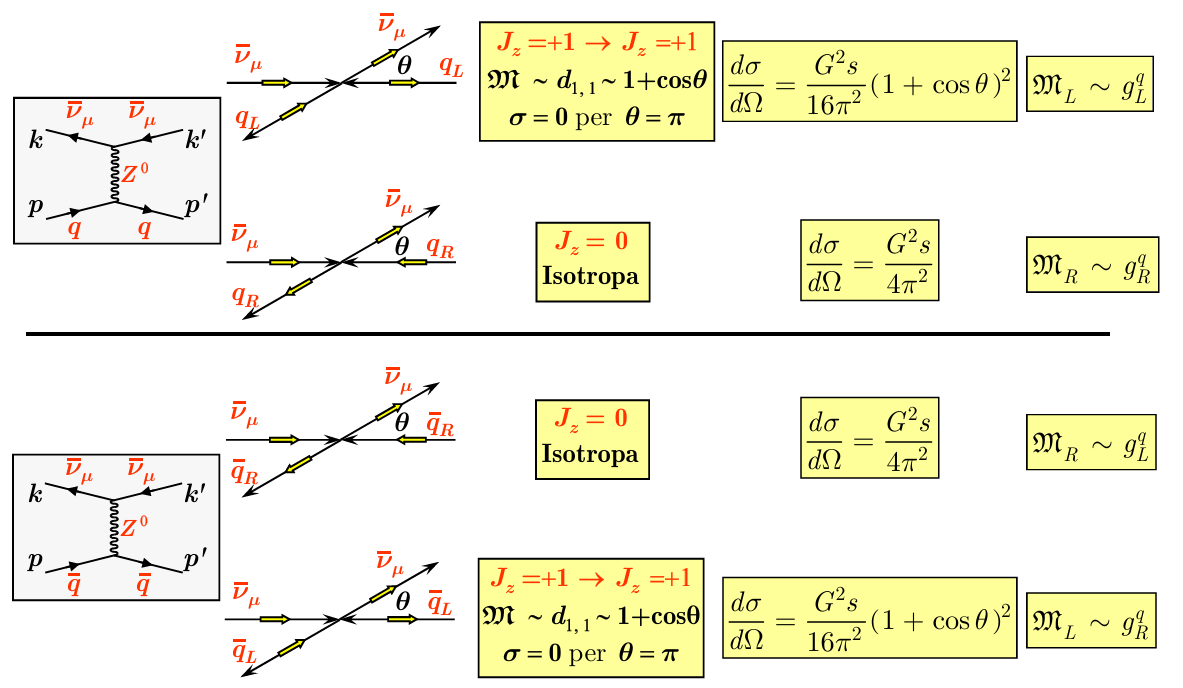
\includegraphics[width=0.4\textwidth]{Lezioni/Lezione 20/salaa3.png}
	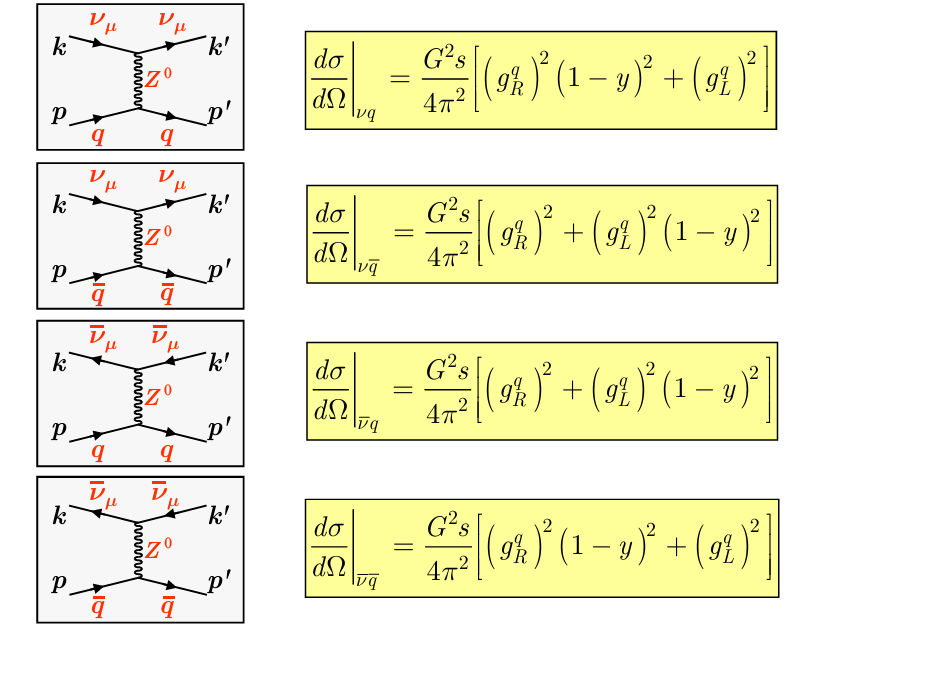
\includegraphics[width=0.4\textwidth]{Lezioni/Lezione 20/salaa4.png}
	\label{fig:salaa3}
\end{figure}
\begin{figure}[h!]
	\centering
	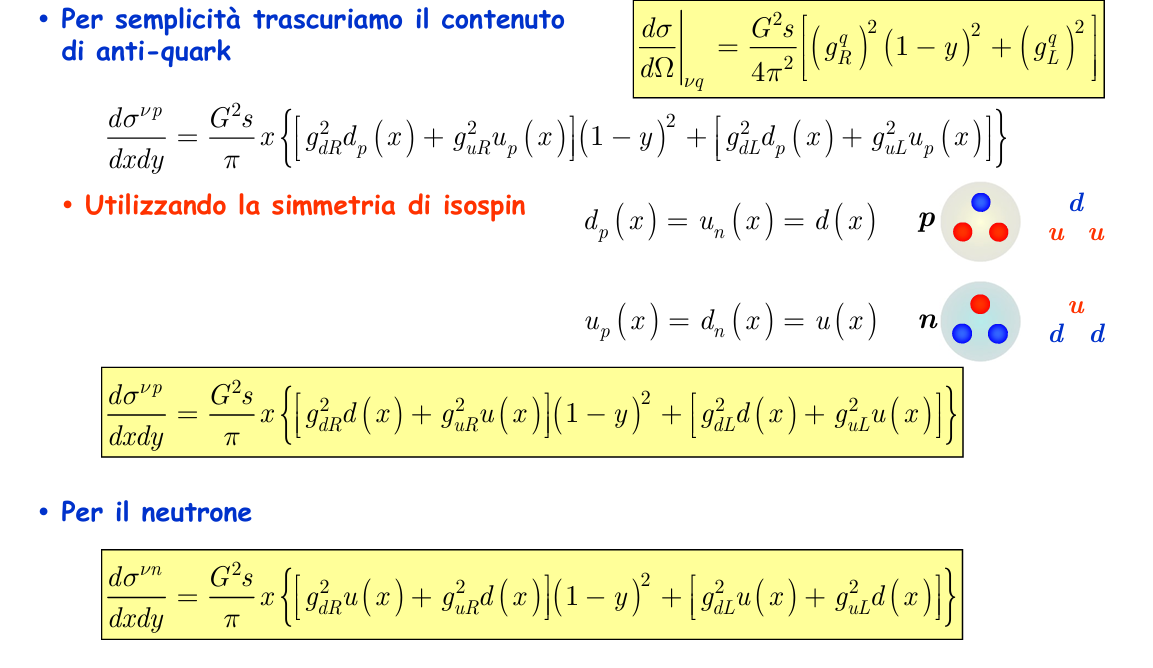
\includegraphics[width=0.4\textwidth]{Lezioni/Lezione 20/salaa5.png}
	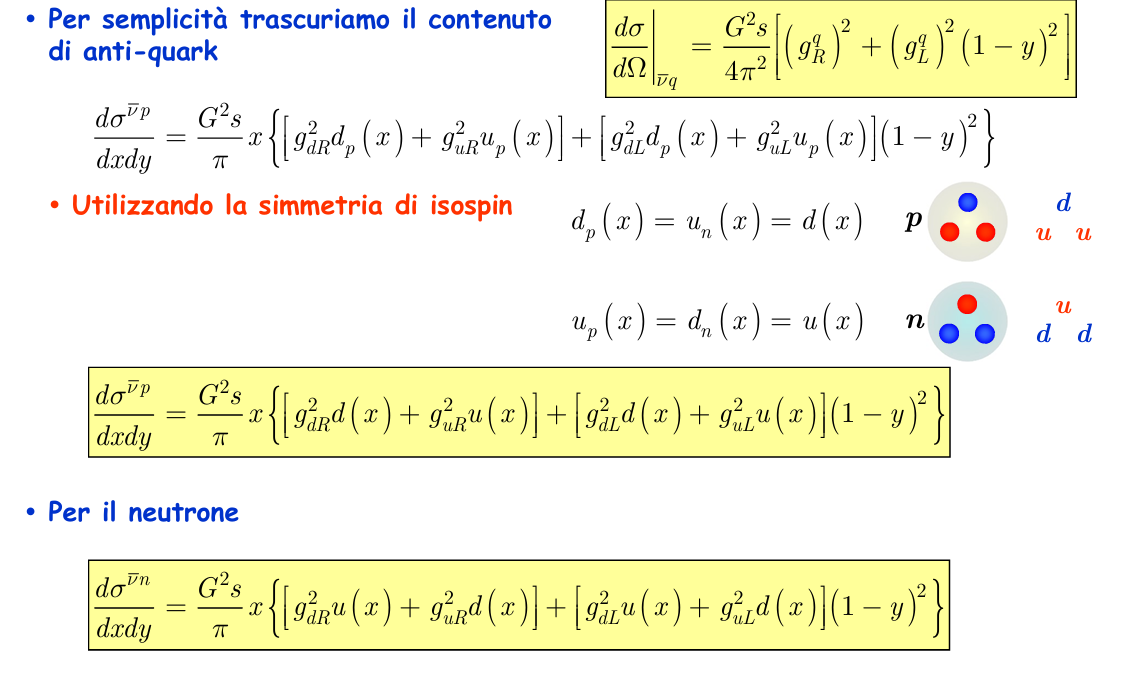
\includegraphics[width=0.4\textwidth]{Lezioni/Lezione 20/salaa6.png}
	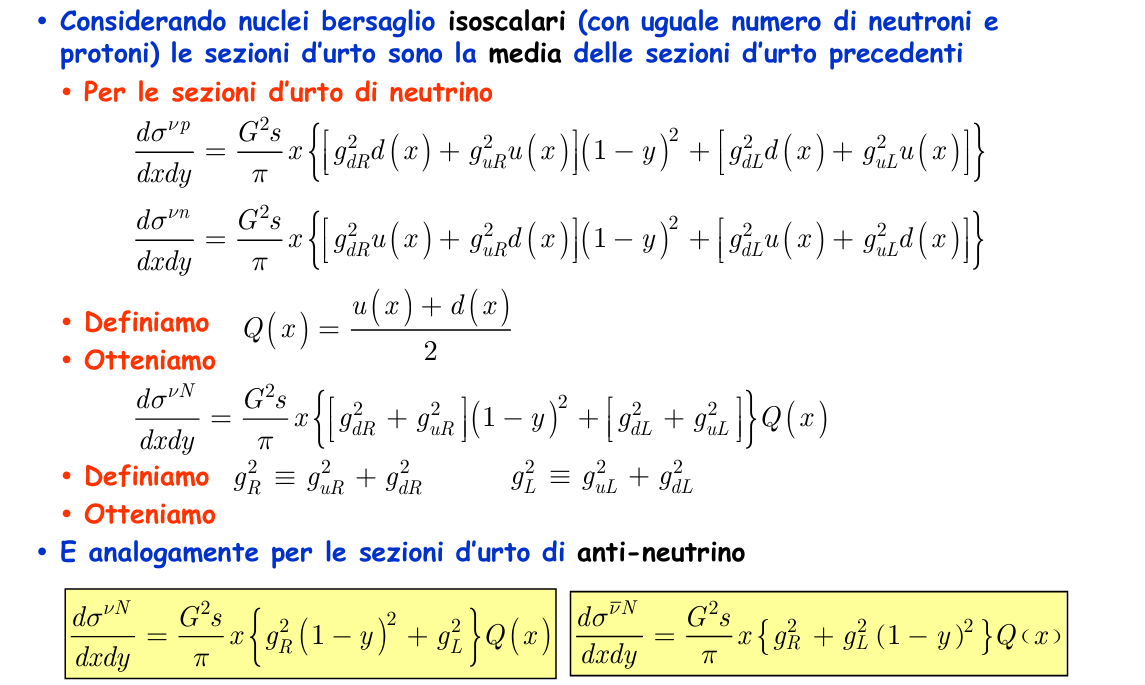
\includegraphics[width=0.4\textwidth]{Lezioni/Lezione 20/salaa7.png}
	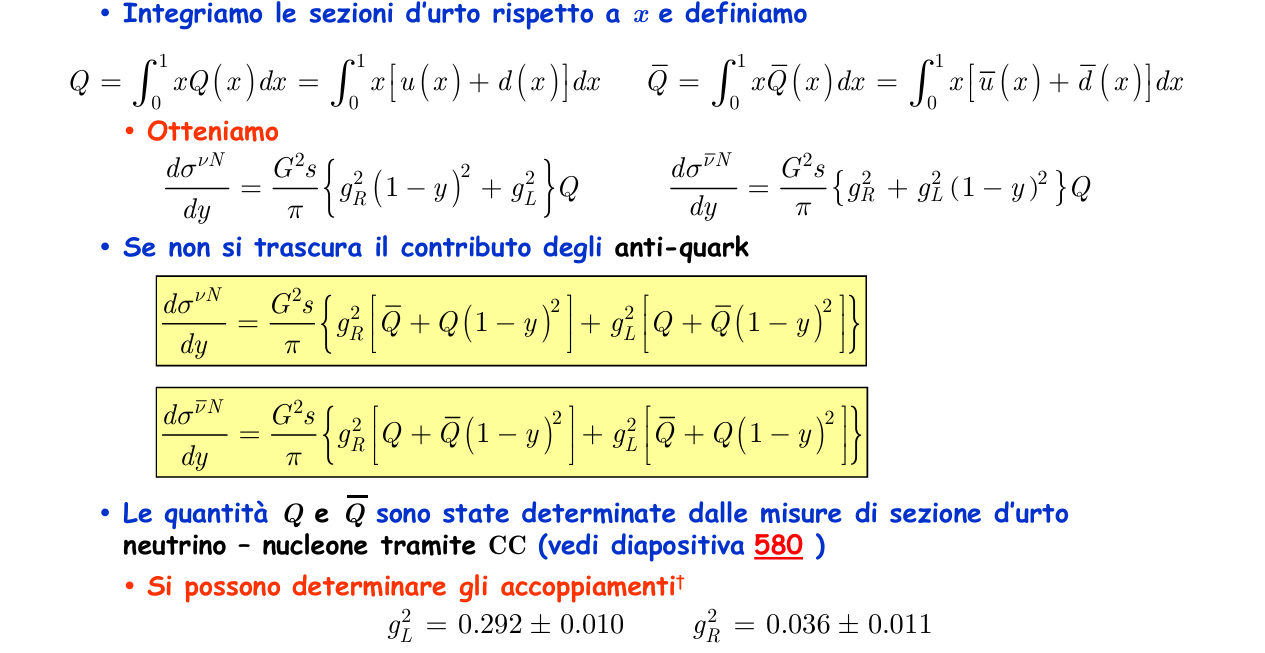
\includegraphics[width=0.4\textwidth]{Lezioni/Lezione 20/salaa8.png}
	\label{fig:salaa5}
\end{figure}
Il risultato assolutamente importante sono le prime misurazioni delle due costanti e cioè
$$
g^2_l=0.292\pm0.010 \qquad g_R^2=0.036\pm0.011
$$
\newpage

\section{Correnti neutre}
Il risultato precedente mostra che le correnti neutre hanno una componente predominante di tipo $V-A$, Hanno comunque una componente $V+A$ non trascurabile. Le misure di interazioni di neutrini tramite corrente neutra sono difficili! Basse sezioni d'urto non si possono misurare le variabilità del leptone nello stato finale e occorre un calorimetro adronico ad alte prestazioni. Gli errori sono anche molto grandi. Sono risultati pre-LEP. Comunque è importante sottolineare che queste misure confermano l'esistenza delle correnti neutre. Hanno mostrato la presenza di una componente $V+A$. Danno un impulso decisivo alla diffusione della teoria di Glashow-Weinberg-Salam.
\section{Interazione neutrino elettrone}
Considerando  le seguenti reazioni:
\begin{itemize}
	\item Neutrino muonico su elettrone procede solo tramite corrente neutra
	$$
	\nu_\mu + e^- \rightarrow \nu_\mu + e^-
	$$
	$$
	\mathfrak{M}_{\nu_\mu e \rightarrow \nu_\mu e} = \frac{G}{\sqrt{2}} \bar{\nu}\gamma^\mu\left(1 - \gamma^5\right)\nu \; \bar{e}\gamma_\mu\left(c_v^e - c_a^e\gamma^5\right)e
	$$
	\item Antineutrino muonico su elettrone procede solo tramite corrente neutra
	$$
	\bar{\nu}_\mu + e^- \rightarrow \bar{\nu}_\mu + e^-
	$$
	\item Per finire la reazione antineutrino elettronico su elettrone che può procedere sia attraverso la corrente neutra che la corrente carica
	$$
	\bar{\nu}_e + e^- \rightarrow \bar{\nu}_e + e^-
	$$
\end{itemize}
\begin{figure}[h!]
	\centering
	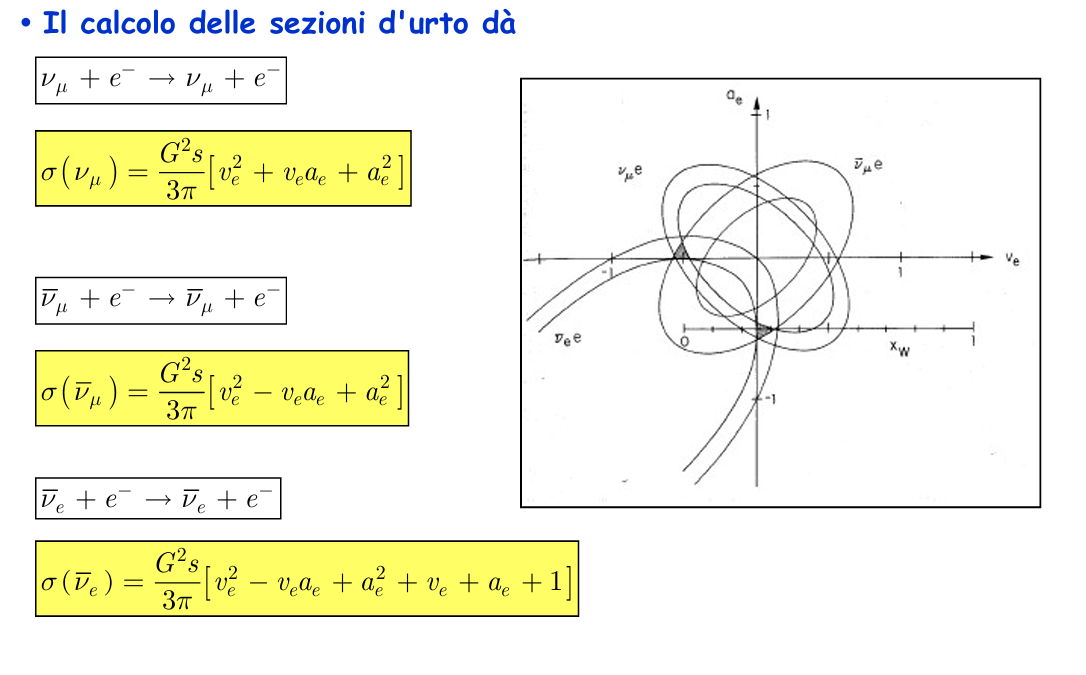
\includegraphics[width=0.4\textwidth]{Lezioni/Lezione 20/sala9.png}
	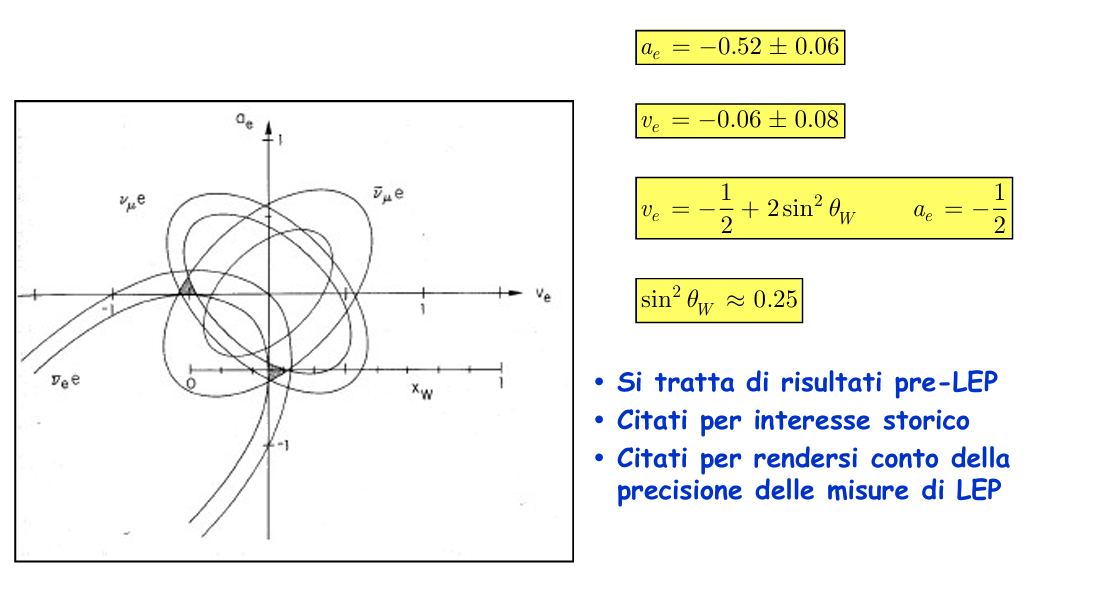
\includegraphics[width=0.4\textwidth]{Lezioni/Lezione 20/sala10.png}
	\label{fig:sala9}
\end{figure}
\begin{figure}[h!]
	\centering
	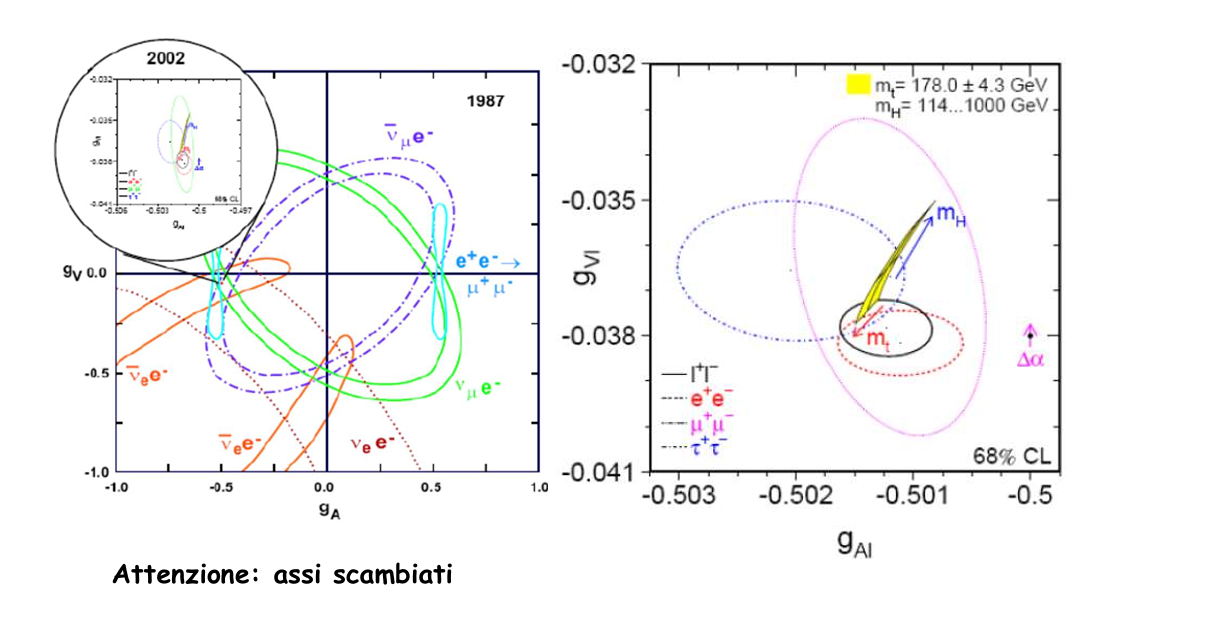
\includegraphics[width=0.9\textwidth]{Lezioni/Lezione 20/sala11.png}
	\label{fig:sala11}
\end{figure}
\section{Le simmetrie del Modello Standard}
L'interazione debole ha correnti cariche e correnti neutre. Richiede mediatori carichi e neutri; ne richiede tre. La corrente carica ha solo la componente chirale $L$ e la corrente neutra ha componenti chirali $L$ e $R$ in misura differente. $SU(2)_L$ non riesce a descrivere la corrente neutra; servono componenti $RH$. L'elettrodinamica è localmente invariante rispetto al gruppo $U(1)$. La corrente elettromagnetica è una corrente neutra e ha componenti chirali $L$ e $R$ presenti in ugual misura. Si introduce un gruppo $U(1)_Y$ chirale che fornisce le componenti mancanti. Il modello standard spiega i fenomeni studiati imponendo una invarianza di gauge locale al gruppo di simmetria sopra introdotto. Infine osserviamo che l'interazione debole ha un range molto breve e quindi i quanti devono avere massa e l'interazione elettromagnetica ha range infinito quindi il mediatore della forza è senza massa (il fotone). Il gruppo proposto da Glashow, Weinberg e Salam soddisfa tutte queste richieste.
\section{Isospin debole}
Le interazioni di corrente di carica dei leptoni che abbiamo studiato sono descritte dalle correnti
\begin{figure}[h!]
	\centering
	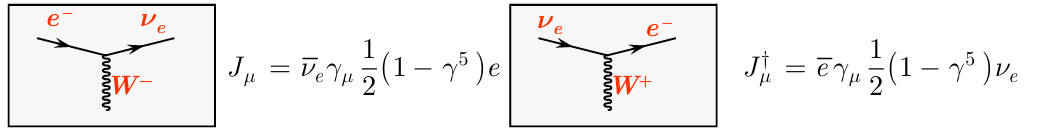
\includegraphics[width=0.9\textwidth]{Lezioni/Lezione 20/sala12.png}
	\label{fig:sala12}
\end{figure}
Introducendo la proiezione chirale le correnti sono riscritte 
$$
f_L = \frac{1}{2}(1 - \gamma^5)f \qquad J_\mu = \bar{\nu}_{eL} \gamma_\mu e_L \quad J_\mu^\dagger = \bar{e}_L \gamma_\mu \nu_{eL}
$$
Correnti analoghe per i quark: transizioni da up a down e viceversa
\begin{figure}[h!]
	\centering
	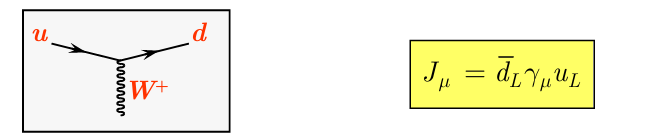
\includegraphics[width=0.6\textwidth]{Lezioni/Lezione 20/sala13.png}
	\label{fig:sala13}
\end{figure}
In analogia a quanto fatto con le correnti di Isospin con $SU(2)$ si possono introdurre dei doppietti (isospinori a due dimensioni)
$$
\ell_L = \begin{pmatrix} \nu_e \\ e \end{pmatrix}_L \qquad q_L = \begin{pmatrix} u \\ d \end{pmatrix}_L
$$
Le proiezioni chirali Left dei fermioni sono pertanto raggruppate in multipletti (doppietti) di isospin debole $T=\frac{1}{2}$
$$
\nu_L \quad T_3=+\frac{1}{2} \qquad e_L \quad T_3=-\frac{1}{2} \qquad u_L \quad T_3=+\frac{1}{2} \qquad d_L \quad T_3=-\frac{1}{2}
$$
Le proiezioni chirali Right dei fermioni sono singoletti di isospin debole $T=0$ $e_R$ $u_R$ $d_R$ $T=0$ mentre $\nu_R$ non esiste (vedremo che è neutro anche per $Y$). L'isospin introdotto, diverso da quello visto per le interazioni forti, si chiama isospin debole ed è la "carica" dell'interazione debole. Le proiezioni chirali Right sono "$SU(2)_L - $ neutre" e quindi non interagiscono con i bosoni $W_1$ $W_2$ $W_3$ associati al gruppo $SU(2)_L$ (e quindi neppure con $W^\pm$). Il gruppo $U(Y)$ introduce diverse quantità di componenti chirali $L$ e $R$ con (più precisamente con intensità di interazione differente). Parte della componente $R$ concorre a formare la componente mancante della corrente debole neutra. La parte rimanente ha uguale "quantità" di componente $L$ e $R$, con simmetria $U(1)$, e forma la corrente elettromagnetica. Descriveremo adesso in dettaglio quanto tratteggiato prima. Vediamo come scrivere le correnti leptoniche e adroniche (quark) in $SU(2)_L$. La simmetria globale $SU(2)_L$ permette di introdurre le correnti conservate $J_i$
$$J_i = \bar{\ell}_L \gamma_\mu \frac{\tau_i}{2} \ell_L$$
Abbiamo usato le matrici di Pauli
$$\begin{aligned}
	\tau_1 = \begin{pmatrix} 0 & 1 \\ 1 & 0 \end{pmatrix} \quad \tau_2 = \begin{pmatrix} 0 & -i \\ i & 0 \end{pmatrix} \quad \tau_3 = \begin{pmatrix} 1 & 0 \\ 0 & -1 \end{pmatrix}
\end{aligned}$$
Definiamo le correnti
$$J_\pm = J_1 \pm iJ_2 \qquad J_\pm = \bar{\ell}_L \gamma_\mu \tau_\pm \ell_L \qquad \begin{aligned}
	\tau_+ = \begin{pmatrix} 0 & 1 \\ 0 & 0 \end{pmatrix} \quad \tau_- = \begin{pmatrix} 0 & 0 \\ 1 & 0 \end{pmatrix}
\end{aligned}$$
La corrente carica leptonica si può scrivere utilizzando $J_+$
$$\begin{aligned}
	J_+ = \bar{\ell}_L \gamma_\mu \tau_+ \ell_L = \begin{pmatrix} \bar{\nu}_e & \bar{e} \end{pmatrix}_L \gamma_\mu \begin{pmatrix} 0 & 1 \\ 0 & 0 \end{pmatrix} \begin{pmatrix} \nu_e \\ e \end{pmatrix}_L = \begin{pmatrix} \bar{\nu}_e & \bar{e} \end{pmatrix}_L \gamma_\mu \begin{pmatrix} e \\ 0 \end{pmatrix}_L = \bar{\nu}_{eL} \gamma_\mu e_L = J_\mu^\dagger
\end{aligned}$$
Analogamente $J_-$ c'è anche la corrente $J_3$
$$J_3 = \bar{\ell}_L \gamma_\mu \frac{\tau_3}{2} \ell_L\qquad J_3 = \frac{1}{2} \bar{\nu}_L \gamma_\mu \nu_L - \frac{1}{2} \bar{e}_L \gamma_\mu e_L$$
Corrisponderebbero ai diagrammi di correnti neutri di tipo V-A fenomeni di corrente neutra di eleettrone puramente V-A non sono mai stati osservati. Quindi dovremo mettere un pezzo di componente Right.

Le correnti $J_i$ con $i=1,2,3$ che abbiamo introdotto sono le correnti di isospin debole. I $3$ bosoni vettoriali $W^k_\mu$ mediano l'interazione, come il fotone $A_\mu$ nella $QED$. In una teoria di gauge gli accoppiamenti delle correnti con i bosoni vettoriali sono fissati dall'invarianza di gauge locale. Per la QED l'invarianza per la trasformazione $e^{i\alpha(x)}$ di $U(1)$ richiede l'introduzione della derivata covariante
$$\partial_\mu \rightarrow D_\mu = \partial_\mu - ieA_\mu(x)$$
Il nuovo termine fissa il vertice di interazione
$$\mathcal{L} = i\bar{\psi}\gamma^\mu\partial_\mu\psi - m\bar{\psi}\psi + e\bar{\psi}\gamma^\mu\psi A_\mu$$
Il gruppo $U(1)$ ha un parametro a cui corrisponde un bosone $A_\mu$. Nel caso dell'isospin debole gli accoppiamenti sono fissati dall'invarianza per trasformazioni locali di $SU(2)_L$
$$\exp\left[i\vec{\alpha}(x)\frac{\vec{\tau}}{2}\right] \qquad D_\mu = \partial_\mu - ig_1\frac{\boldsymbol{\tau}}{2} \cdot \mathbf{W}_\mu(x)$$
Il gruppo $SU(2)_L$ ha 3 parametri a cui corrispondono 3 bosoni $W^k$. Con $D_\mu$ la lagrangiana diventa
$$\mathcal{L} = i\bar{\ell}\gamma^\mu\partial_\mu\ell - m\bar{\ell}\ell + g_1\bar{\ell}\gamma^\mu\frac{\boldsymbol{\tau}}{2} \cdot \mathbf{W}_\mu\ell$$
Abbiamo visto che la corrente mediata da $W^3$ non corrisponde a fenomeni osservati
$$J_3 = \frac{1}{2}\bar{\nu}_L\gamma_\mu\nu_L - \frac{1}{2}\bar{e}_L\gamma_\mu e_L$$
ça distribuzione angolare delle interazioni di corrente neutra di neutrini con elettroni e quarks mostra che non sono correnti $V-A$. Sappiamo che sperimentalmente si osserva che le correnti neutre dei fermioni carichi hanno una componente $V-A$ che una $V+A$
$$J_\mu^{NC} = g_R\bar{e}_R\gamma_\mu e_R + g_L\bar{e}_L\gamma_\mu e_L$$
Abbiamo osservato che la corrente elettromagnetica ha sia comportamenti LH che RH che interagiscono allo stesso modo
$$J_\mu^{em} = -e\bar{u}\gamma_\mu u = -e\bar{u}_R\gamma_\mu u_R - e\bar{u}_L\gamma_\mu u_L$$
Pertanto da questa osservazione si introduce il gruppo $U(1)_Y$ per introdurre ulteriori componenti $f_R$ e $f_L$, con interazioni differenti per
\begin{itemize}
	\item Costruire una corrente neutra elettromagnetica (con uguale presenza di componenti $R$ e $L$)
	\item  Costruire una corrente neutra debole (che riporduca le componenti $V+A$ e $V-A$ osservate)
\end{itemize}
\section{Il modello standard}
Il gruppo di simmetria (a 4 parametri) del modello standard è $SU(2)_L\otimes U(1)_Y$. Ai due gruppi sono associati i seguenti bosoni vettoriali
$$\text{SU}(2)_{\text{L}} \qquad W_1^\mu, W_2^\mu, W_3^\mu \qquad \text{U}(1)_{\text{Y}} \qquad B^\mu$$
Il gruppo $U(1)_Y$ è associato ad un ulteriore numero quantico. L'ipercarica debole, cui è associata una corrente di ipercarica debole. Analoga alla corrente $U(1)_Q$ dell'elettromagnetismo
$$J_Y^\mu = \bar{f} \gamma^\mu Y f$$
Tuttavia $Y$ differenzia le componenti $f_R$ e $f_L$. La relazione tra isospin debolem ipercarica debole e carica è identica alla relazione di Gell-Mann e Nishijima. Questa relazione ci dice che con una opportuna scelta di $Y$, esiste una combinazione di correnti di isospin debole e di corrente di ipercarica debole che riproduce la corrente elettromagnetica.
$$\frac{Q}{e} = T_3 + \frac{Y}{2}$$
\begin{figure}[h!]
	\centering
	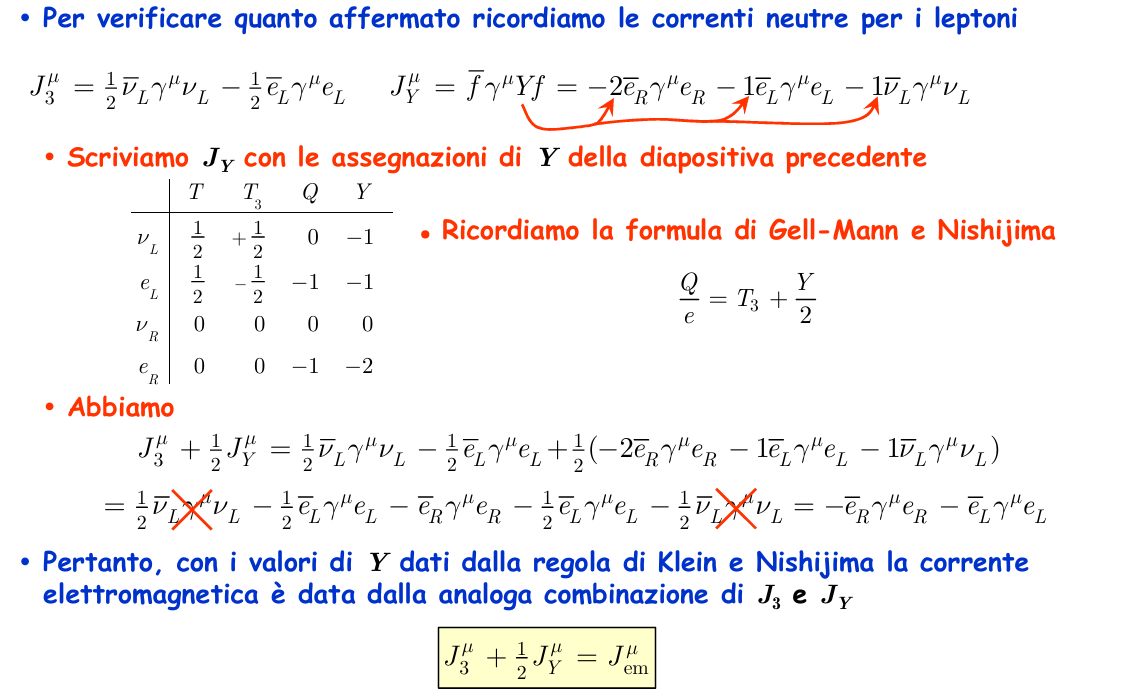
\includegraphics[width=0.9\textwidth]{Lezioni/Lezione 20/sala14.png}
	\label{fig:sala14}
\end{figure}
\section{Scomposizione chirale della $\mathcal{L}$ di Dirac}
Ricordiamo i proiettori chirali e le loro principali rpoprietà
$$P_R = \frac{1}{2}(1 + \gamma^5) \qquad P_L = \frac{1}{2}(1 - \gamma^5) \qquad P_L P_R = 0 \qquad P_X P_X = P_X \qquad P_R + P_L = I$$
Introduciamo le proiezioni chirali dei campi
$$\psi_R = P_R \psi \qquad \psi_L = P_L \psi \qquad \bar{\psi}_R = \overline{P_R \psi} = (P_R \psi)^\dagger \gamma^0 = \psi^\dagger P_R \gamma^0 = \psi^\dagger \gamma^0 P_L = \bar{\psi} P_L$$
E analogamente per la proiezione $R$
$$\bar{\psi}_R = \bar{\psi} P_L \qquad \bar{\psi}_L = \bar{\psi} P_R$$
La lagrangiana libera è scritta con i campi completi
$$\mathcal{L} = i\bar{\psi}\gamma^\mu\partial_\mu\psi - m\bar{\psi}\psi$$
Consideriamo il termine cinetico
$$\bar{\psi}\gamma^\mu\partial_\mu\psi = (\bar{\psi}_R + \bar{\psi}_L)\gamma^\mu\partial_\mu(\psi_R + \psi_L) = \bar{\psi}_R\gamma^\mu\partial_\mu\psi_R + \cancel{\bar{\psi}_R\gamma^\mu\partial_\mu\psi_L} + \bar{\psi}_L\gamma^\mu\partial_\mu\psi_L + \cancel{\bar{\psi}_L\gamma^\mu\partial_\mu\psi_R}$$
I termini "incrociati" sono nulli
$$\bar{\psi}_R\gamma^\mu\partial_\mu\psi_L = \bar{\psi} P_L \gamma^\mu \partial_\mu P_L \psi = \bar{\psi}\gamma^\mu P_R \partial_\mu P_L \psi = 0$$
In conclusione
$$\bar{\psi}\gamma^\mu\partial_\mu\psi = \bar{\psi}_R\gamma^\mu\partial_\mu\psi_R + \bar{\psi}_L\gamma^\mu\partial_\mu\psi_L$$
Per il termine di massa il comportamento è diverso
$$\begin{aligned}
	\bar{\psi}\psi &= (\bar{\psi}_R + \bar{\psi}_L)(\psi_R + \psi_L) = \bar{\psi}_R\psi_R + \bar{\psi}_L\psi_R + \bar{\psi}_R\psi_L + \bar{\psi}_L\psi_L \\
	&= \cancel{\bar{\psi} P_L P_R \psi} + \bar{\psi} P_L P_L \psi + \bar{\psi} P_R P_R \psi + \cancel{\bar{\psi} P_R P_L \psi} = \bar{\psi}_L\psi_R + \bar{\psi}_R\psi_L
\end{aligned}$$
In conclusione
$$\bar{\psi}\psi = \bar{\psi}_L\psi_R + \bar{\psi}_R\psi_L$$
Riassumiamo il risultato ottenuto
$$\mathcal{L} = i\bar{\psi}\gamma^\mu\partial_\mu\psi - m\bar{\psi}\psi = i\bar{\psi}_R\gamma^\mu\partial_\mu\psi_R + i\bar{\psi}_L\gamma^\mu\partial_\mu\psi_L - m(\bar{\psi}_L\psi_R + \bar{\psi}_R\psi_L)$$
Osserviamo che il termine cinetico non mescola le due proiezioni chirali e il termine di massa mescola le due proiezioni chirali. Pertanto, ai fini delle invarianze il termine cinetico mantiene la sua invarianza anche se le propiezioni $R$ e $L$ si comportano in modo differente. Il termine di massa non è invariante se le due proiezioni $R$ e $L$ si comportnato in modo differente. Se le proieizoni chirali $R$ e $L$ hanno comportamento diverso, per avere una teoria invariante la massa dei fermioni deve essere nulla. Conseguenza della natura "chirale" della teoria. Vedremo che è possibile dare la massa dinamicamente tramite il bosone di Higgs.
\section{Il modello standard}
L'invarianza locale di Gauge fissa gli accoppiamenti Bosoni-Correnti
$$D_\mu = \partial_\mu + ig_1 \frac{\boldsymbol{\tau}}{2} \cdot \mathbf{W}_\mu(x) + ig_2 \frac{Y}{2} B_\mu \quad \mathcal{L}' = g_1 \left( J_1^\mu W_\mu^1 + J_2^\mu W_\mu^2 + J_3^\mu W_\mu^3 \right) + \frac{1}{2} g_2 J_Y^\mu B_\mu$$
I parametri $g_1$ e $g_2$ sono le costanti di accoppiamento relative ai gruppi $SU(2)_L$ e $U(1)_Y$ rispettivamente. I bosoni vettoriali $W$ e $B$ hanno massa nulla (teoria rinormalizzabile). Per dotare i bosoni di massa Weinberg e Salam introdussero nella teoria il meccanismo della rottura spontanea della simmetria. Introduzione di un doppietto scalare: il campo di Higgs, invarianza locale della lagrangiana del campo di Higgs e rottura spontanea della simmetria. Vedremo che tramite la rottura della simmetria i bosoni $W^3$ e $B$ sono sostituiti dalle combinazioni lineare ()$M_A=0, M_Z$). Anticipiamo il risultato
$$\begin{aligned}
	A_\mu &= B_\mu \cos\theta_W + W_\mu^3 \sin\theta_W \\
	Z_\mu &= -B_\mu \sin\theta_W + W_\mu^3 \cos\theta_W
\end{aligned}$$
\section{Correnti cariche}
Le correnti accoppiate ai bosoni $W^1$ e $W^2$ sono
$$g_1(J_1^\mu W_\mu^1 + J_2^\mu W_\mu^2)$$
Utilizzando l'isospin debole abbiamo definito le correnti
$$J_+ = J_1 + iJ_2 \quad J_- = J_1 - iJ_2 \qquad J_1 = \frac{1}{2}(J_+ + J_-) \quad J_2 = \frac{i}{2}(J_- - J_+)$$
Sostituendo $J_1$ e $J_2$ nella prima espressione
$$\frac{g_1}{2} \left( (J_+^\mu + J_-^\mu)W_\mu^1 + i(J_-^\mu - J_+^\mu)W_\mu^2 \right) \qquad \frac{g_1}{2} \left( J_+^\mu(W_\mu^1 - iW_\mu^2) + J_-^\mu(W_\mu^1 + iW_\mu^2) \right)$$
Definiamo i nuovi bosoni $W^+$ e $W^-$
$$W_\mu^+ = \frac{W_\mu^1 - iW_\mu^2}{\sqrt{2}} \qquad W_\mu^- = \frac{W_\mu^1 + iW_\mu^2}{\sqrt{2}}$$
Vedremo che le combinazioni $W^+$ e $W^-$ hanno massa $M_W$. Sostituendo otteniamo
$$\frac{g_1}{\sqrt{2}} \left( J_+^\mu W_\mu^+ + J_-^\mu W_\mu^- \right)$$
Queste sono le interazioni di correnti cariche che abbiamo studiato e hanno la struttura $V-A$.
\section{Corrente elettromagnetica: Isospin + Ipercarica}
Interpretiamo adesso le correnti neutre
$$J_\mu^Y = Y_{eR}\bar{e}_R\gamma_\mu e_R + Y_{eL}\bar{e}_L\gamma_\mu e_L + Y_{\nu L}\bar{\nu}_L\gamma_\mu\nu_L \qquad J_3 = \frac{1}{2}\bar{\nu}_L\gamma_\mu\nu_L - \frac{1}{2}\bar{e}_L\gamma_\mu e_L$$
Gli accoppiamenti sono
$$g_1 J_3^\mu W_\mu^3 + \frac{1}{2} g_2 J_Y^\mu B_\mu$$
Sostituiamo la definizione dei Bosoni Neutri ottenuti dopo la rottura spontanea della simmetria
$$B_\mu = A_\mu \cos\theta_W - Z_\mu \sin\theta_W \qquad W_\mu^3 = A_\mu \sin\theta_W + Z_\mu \cos\theta_W$$
Otteniamo
$$g_1 J_3^\mu W_\mu^3 + \frac{1}{2} g_2 J_Y^\mu B_\mu = g_1 J_3^\mu A_\mu \sin\theta_W + g_1 J_3^\mu Z_\mu \cos\theta_W + \frac{1}{2} g_2 J_Y^\mu A_\mu \cos\theta_W - \frac{1}{2} g_2 J_Y^\mu Z_\mu \sin\theta_W$$
Consideriamo dapprima le correnti accoppiate ad $A_\mu$. Sostituendo le $J$
$$\frac{1}{2} g_1 \left( \bar{\nu}_L \gamma^\mu \nu_L - \bar{e}_L \gamma^\mu e_L \right) A_\mu \sin\theta_W + \frac{1}{2} g_2 \left( Y_{eR} \bar{e}_R \gamma^\mu e_R + Y_{eL} \bar{e}_L \gamma^\mu e_L + Y_{eL} \bar{\nu}_L \gamma^\mu \nu_L \right) A_\mu \cos\theta_W$$
Sostituiamo i valori dell'ipercarica $Y_{eL}=Y_{\nu L}=-1$ e $Y_{eR}=-2$
$$\frac{1}{2} \left( g_1 \sin\theta_W \bar{\nu}_L \gamma^\mu \nu_L - g_1 \sin\theta_W \bar{e}_L \gamma^\mu e_L - 2g_2 \cos\theta_W \bar{e}_R \gamma^\mu e_R - g_2 \cos\theta_W \bar{e}_L \gamma^\mu e_L - g_2 \cos\theta_W \bar{\nu}_L \gamma^\mu \nu_L \right) A_\mu$$
Sappiamo che il fotone non si accoppia al neutrino e quindi bisogna eliminare i termini con i campi $\nu_L$. Per eliminare i termini con i neutrini è sufficiente porre
$$g_1 \sin\theta_W = g_2 \cos\theta_W$$
Sopravvivono i termini
$$\frac{1}{2} \left( -g_1 \sin\theta_W \bar{e}_L \gamma^\mu e_L - 2g_2 \cos\theta_W \bar{e}_R \gamma^\mu e_R - g_2 \cos\theta_W \bar{e}_L \gamma^\mu e_L \right) A_\mu$$
Perchè questa sia la corrente elettromagnetica gli accoppiamenti di $e_L$ e $e_R$ devono essere uguali fra loro e uguali alla carica dell'elettrone $e$
$$-g_1 \sin\theta_W - g_2 \cos\theta_W = -2g_2 \cos\theta_W$$
Otteniamo infine
$$g_1 \sin\theta_W = g_2 \cos\theta_W = e$$
Sostituendo
$$\frac{1}{2} \left( -e\bar{e}_L \gamma^\mu e_L - 2e\bar{e}_R \gamma^\mu e_R - e\bar{e}_L \gamma^\mu e_L \right) A_\mu = -e(\bar{e}_L \gamma^\mu e_L + \bar{e}_R \gamma^\mu e_R) A_\mu$$
Contiene componeneti $R$ e $L$ in egual misura e abbiamo ritrovato la interazione elettromagnetica.
\begin{figure}[h!]
	\centering
	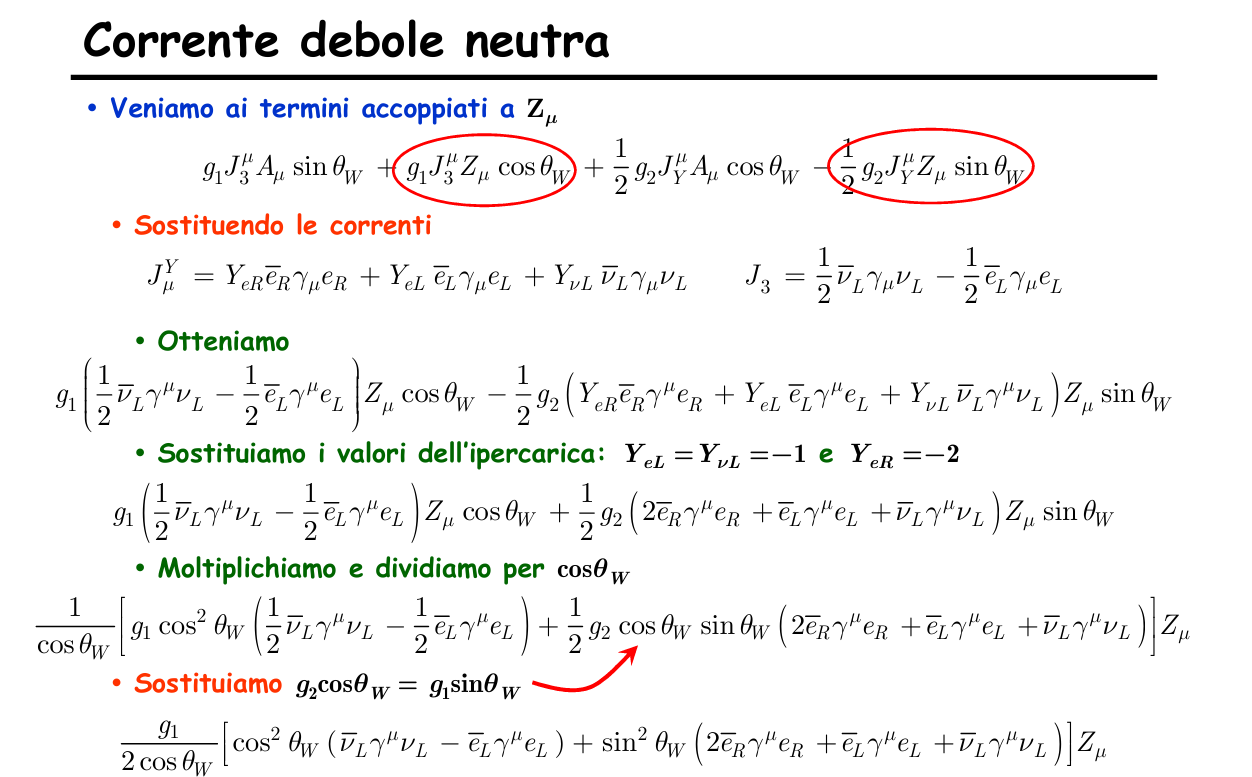
\includegraphics[width=0.4\textwidth]{Lezioni/Lezione 20/sala15.png}
	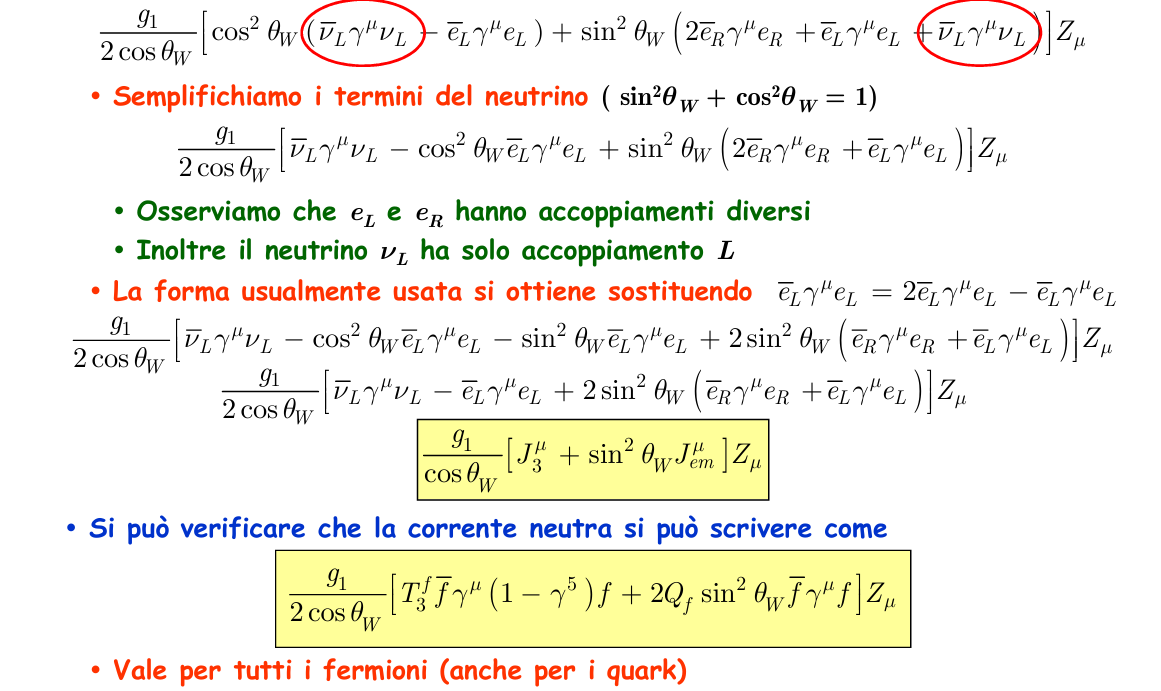
\includegraphics[width=0.4\textwidth]{Lezioni/Lezione 20/sala17.png}
	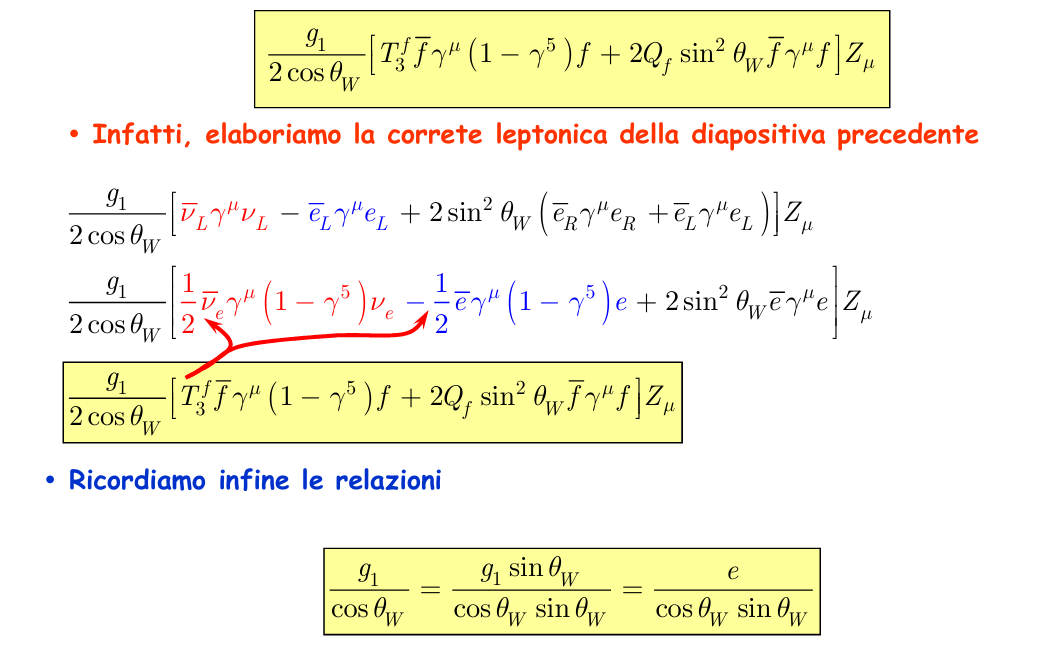
\includegraphics[width=0.4\textwidth]{Lezioni/Lezione 20/sala18.png}
	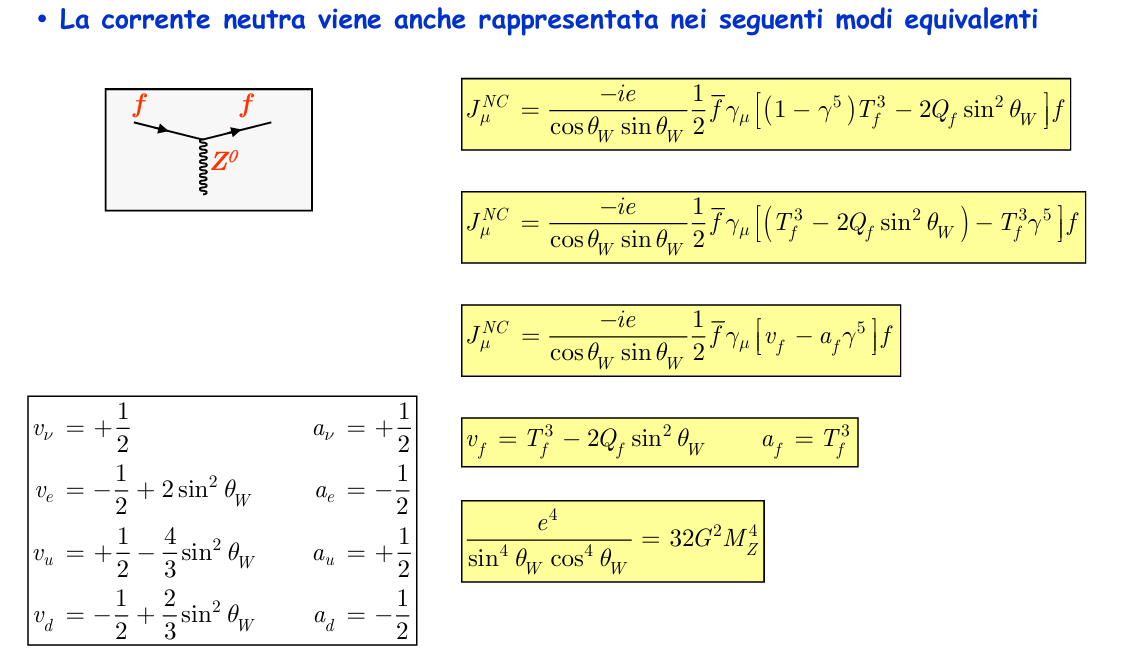
\includegraphics[width=0.4\textwidth]{Lezioni/Lezione 20/sala19.png}
	\label{fig:sala19}
\end{figure}